% This is "www2010-sample.tex" copied from "www2005-sample.tex" V1.2 January 26 2004
% This file should be compiled with V1.4 of "www2010-submission.class"
%
% This example file demonstrates the use of the 'www2010-submission.cls'
% V1.4 LaTeX2e document class file. It is for those submitting
% articles to the WWW'04 Conference WHO DO NOT WISH TO
% STRICTLY ADHERE TO THE SIGS (PUBS-BOARD-ENDORSED) STYLE.
% The 'www2010-submission.cls' file will produce a similar-looking,
% albeit, 'tighter' paper resulting in, invariably, fewer pages.
%
% ----------------------------------------------------------------------------------------------------------------
% This .tex file (and associated .cls V1.4) produces:
%       1) NO Permission Statement
%       2) WWW'04-specific conference (location) information
%       3) The Copyright Line with ACM data
%       4) NO page numbers
%
% ---------------------------------------------------------------------------------------------------------------
% This .tex source is an example which *does* use
% the .bib file (from which the .bbl file % is produced).
% REMEMBER HOWEVER: After having produced the .bbl file,
% and prior to final submission, you *NEED* to 'insert'
% your .bbl file into your source .tex file so as to provide
% ONE 'self-contained' source file.
%
% ================= IF YOU HAVE QUESTIONS =======================
% Questions regarding the SIGS styles, SIGS policies and
% procedures, Conferences etc. should be sent to
% Julie Goetz (goetz@acm.org) or Adrienne Griscti (griscti@acm.org)
%
% Technical questions only to
% Gerald Murray (murray@acm.org)
% ===============================================================
%
% For tracking purposes - this is V1.2 - January 26 2004
\documentclass{www2010-submission}

\begin{document}
%
\title{Search the Web Using GUI Screenshots}
%\subtitle{[Extended Abstract]
%\titlenote{A full version of this paper is available as
%\textit{Author's Guide to Preparing ACM SIG Proceedings Using
%\LaTeX$2_\epsilon$\ and BibTeX} at
%\texttt{www.acm.org/eaddress.htm}}}
%
% You need the command \numberofauthors to handle the "boxing"
% and alignment of the authors under the title, and to add
% a section for authors number 4 through n.
%
% Up to the first three authors are aligned under the title;
% use the \alignauthor commands below to handle those names
% and affiliations. Add names, affiliations, addresses for
% additional authors as the argument to \additionalauthors;
% these will be set for you without further effort on your
% part as the last section in the body of your article BEFORE
% References or any Appendices.

\numberofauthors{2}
%
% Put no more than the first THREE authors in the \author command

% NOTE: All authors should be on the first page. For instructions
% for more than 3 authors, see:
% http://www.acm.org/sigs/pubs/proceed/sigfaq.htm#a18





\author{
%
% The command \alignauthor (no curly braces needed) should
% precede each author name, affiliation/snail-mail address and
% e-mail address. Additionally, tag each line of
% affiliation/address with \affaddr, and tag the
%% e-mail address with \email.
\alignauthor Tom Yeh, Brandyn White, Larry Davis\\
       \affaddr{University of Maryland}\\
       \affaddr{College Park, MD, USA}\\
       \email{\{tomyeh, bwhite, lsd\}@umd.edu}
%\alignauthor Brandyn White\\
%       \affaddr{Institute for Clarity in Documentation}\\
%       \affaddr{P.O. Box 1212}\\
%       \affaddr{Dublin, Ohio 43017-6221}\\
%       \email{webmaster@marysville-ohio.com}
%\alignauthor Larry S. Davis\\
%       \affaddr{Institute for Clarity in Documentation}\\
%       \affaddr{P.O. Box 1212}\\
%       \affaddr{Dublin, Ohio 43017-6221}\\
%       \email{webmaster@marysville-ohio.com}
\alignauthor Boris Katz\\
       \affaddr{CSAIL}\\
       \affaddr{Cambridge, MA, USA}\\
       \email{boris@mit.edu}
}
\additionalauthors{Additional authors: John Smith (The Th{\o}rv\"{a}ld Group,
email: {\texttt{jsmith@affiliation.org}}) and Julius P.~Kumquat
(The Kumquat Consortium, email: {\texttt{jpkumquat@consortium.net}}).}
\date{30 July 1999}
%\begin{figure*}[t]
%
\includegraphics[width=2\columnwidth]{authors.png}
%\end{figure*}
\maketitle

\begin{abstract}
This paper provides a sample of a LaTeX document which conforms,
somewhat loosely, to the formatting guidelines for
ACM SIG Proceedings. It is an {\em alternate} style which produces
a {\em tighter-looking} paper and was designed in response to
concerns expressed, by authors, over page-budgets.
It complements the document \textit{Author's (Alternate) Guide to
Preparing ACM SIG Proceedings Using \LaTeX$2_\epsilon$\ and Bib\TeX}.
This source file has been written with the intention of being
compiled under \LaTeX$2_\epsilon$\ and BibTeX.
The developers have tried to include every imaginable sort
of ``bells and whistles", such as a subtitle, footnotes on
title, subtitle and authors, as well as in the text, and
every optional component (e.g. Acknowledgments, Additional
Authors, Appendices), not to mention examples of
equations, theorems, tables and figures.
To make best use of this sample document, run it through \LaTeX\
and BibTeX, and compare this source code with the printed
output produced by the dvi file. A compiled PDF version
is available on the web page to help you with the
`look and feel'.
\end{abstract}

% A category with only the three required fields
\category{H.4.m}{Information Systems}{Miscellaneous}
\category{D.2}{Software}{Software Engineering}
%A category including the fourth, optional field follows...
\category{D.2.8}{Software Engineering}{Metrics}[complexity measures,
performance measures]

\terms{Image search}

\keywords{Image search}

\section{Introduction}

There are a lot of resources on the Web about software
applications. Users can learn from these resources teach how to
perform a wide variety of tasks such as setting up a home network,
backing up files, or changing the speed of the mouse cursor. These
resources are often created and made available online by software
developers themselves who wish to maintain an online version of
the documentation apart from the built-in one in order to keep the
content always up-to-date (e.g., support.microsoft.com). These
resources are also created by unofficial, third-party experts, for
example, by sites offering tutorials and tips on various software
applications (e.g., osxfaq.com), by general-purpose \emph{how-to}
sites (e.g., eHow.com) featuring software tutorials as one of the
topics, and by computer book publishers who wish to make their
books accessible online via subscription (e.g.,
safaribooksonline.com). Even more resources can be found in
user-generated contents, for example, in blogs where bloggers
share their experiences and tips using the software application,
in discussion boards where people can discuss and learn from each
other about software, and in QA communities such as Yahoo Answers
where members can raise question and get answers back from other
members.

However, for some users, searching this valuable resource
effectively can be challenging. For example, suppose a user opens
up the network properties dialog window and wishes to find out how
to change the IP address. To use a search engine, this user may
first type ``change IP address'' to describe the task he wishes to
learn. He may soon realize it is also necessary to indicate which
dialog window he wishes to perform the task with. To do so, he may
enter additional search terms to describe the operating system,
the title of the dialog window, and any other information needed
to identify the dialog window. Not only is it \textbf{cumbersome
to enter many keywords} but also these keywords are \textbf{prone
to ambiguity} since it is hard distinguish the keywords describing
the program from those describing the task. Moreover, as the user
browses the links in the result, the user may find it
\textbf{difficult to judge relevancy} based only on the summary
text. The emphasis on second language education and the
availability of free and powerful machine translation technology
(e.g., Google Translate) have enabled many Web users to perform
bilingual search in order to access more information beyond the
confine of their native languages. However, technical articles are
often \textbf{inaccessible by bilingual search}. For example, a
Chinese-speaking person fluent in English may be able to retrieve
useful articles on dogs in both languages using the English or
Chinese word for \emph{dog} as the search term. But when it comes
to technical terms such as \emph{system preferences}, the same
person may be confined to only Chinese articles since it is not
obvious how to translate these terms into English.


%Users often rely on the names displayed on the interface to
%describe keywords. Many non-English speaking users use localized
%software in their native language. They can read and understand
%English well or use a machine translator such as Babel to help
%them understand. While translating common terms is easy,
%translating technical interface names is hard, making the
%English-language resources inaccessible to these international
%users.


(The ranking in this example has been artificially adjusted in
order to illustrate a rich variety of results.)

\begin{figure*}
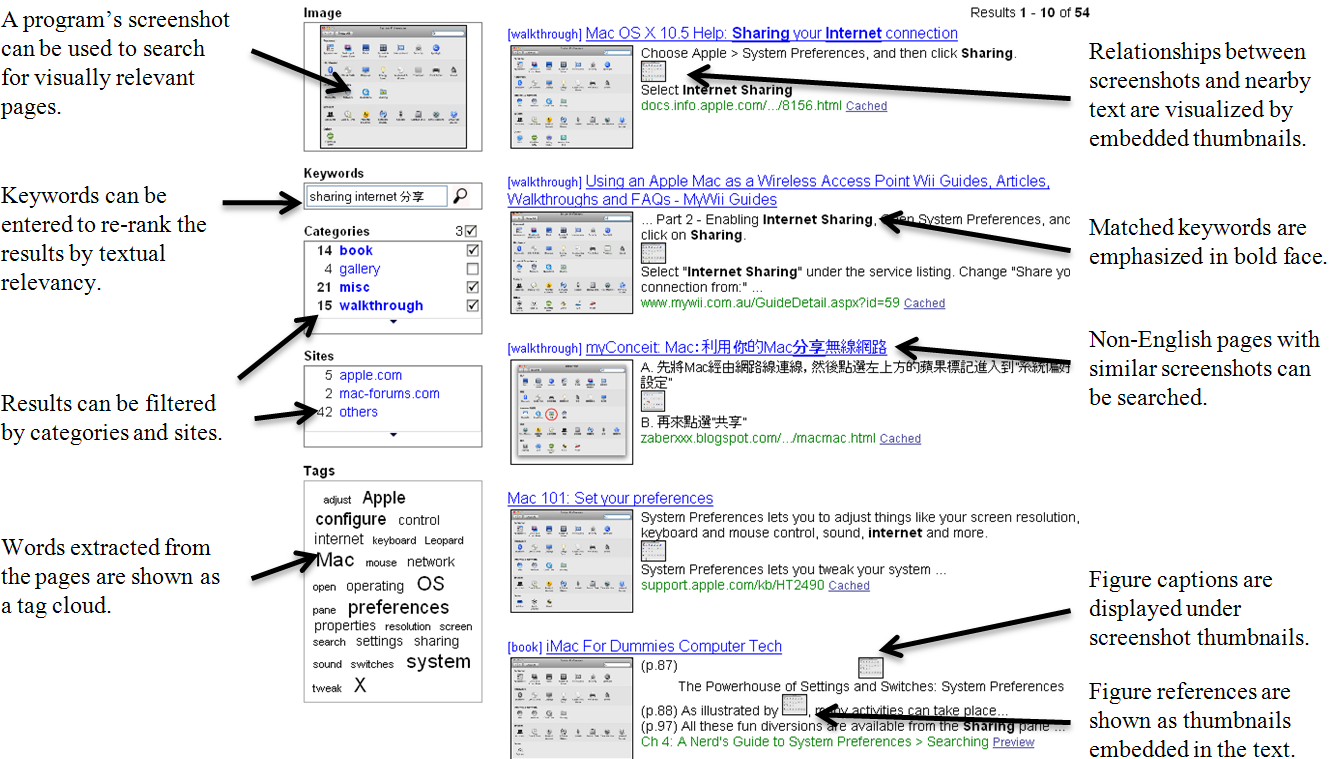
\includegraphics[width=2\columnwidth]{figure/main_result.png}
\end{figure*}

%One possibility is to choose the words at the title of the window
%as keywords. The user also needs to specify what a
%
%* Need to type many keywords. Most cases copy and paste is not supported.
%* Ambiguity: how to do X with Y? But keywords are all the same.
%* Hard to judge the relevancy.
%* Sometimes in a long document with multiple steps, it's unclear
%where in the document is relevant to the current screen.
%* can not search cross langauge (bi-lingual who may be familiar
%with the terms in one language but can read the explanation in two
%languages equally well)

C: Use multi-modal search
    Brief system demo
        walk through a search scenario
        showoff the scale
    Explain how each limitation is overcome
    List of contributions
        Propose a new large-scale search system
        Evaluate it
    Road map

\section{Related Work}
    WWW citations about image search
    Vision citations

\section{Challenges}

\section{Building the database}

\subsection{Collecting images}

%With lots of resources like a commercial search companies, it is
%possible to crawl the web and collect a large number of
%screenshots. As an academic research project, we are limited by
%resource. Yet, we still manage to build a research prototype
%database at a non-trivial scale of 100,000 images. These images
%came from three sources.

We used three methods to collect screenshot images to populate our
database. Currently, our prototype system contains a total of
150,000 images in its index.

First, we submitted computer-related keywords to Bing Image Search
to collect screenshot images of interactive programs. To increase
the likelihood of obtaining the desired images, we sampled
keywords from title bars of the dialog windows of various computer
programs. Some examples of these keywords are properties,
preferences, option, settings, wizard, custom, installation,
network, sound, keyboard ....etc. We turned on the filter feature
to keep only illustration and graphics, rejecting obviously
non-screenshot images such as images of faces and natural scenes.
Using this method, we collected a total of 100,000 images, about
80\% of them are screenshots of computer programs.

Second, we used TinEye, a reverse image search engine that can
take an image as the query and return a list of URLs to nearly
identical copies of the image found on the Web for copyright
infringement. We manually captured screenshot images of more than
300 interactive windows of popular programs across three of the
most popular OS platforms (XP, Vita, and Mac OS). These images
were submitted to TinEye to obtain about 5,000 images. Since the
visual similarity matching performed by TinEye is very precise,
all of these images are screenshot images.

Third, we collected a library of 102 electronic books on popular
software programs. We extracted all the image figures embedded in
the electronic file (i.e., Pdf documents). About x\% of these
figures are screenshots. This method gave us about 50,000 images.

Each method has its own pros and cons. While Bing Image Search
provides the best variety of images, many of them are not visually
relevant to any program at all. TinEye is able to provide visually
relevant images. But these images are ranked only by visual
relevancy; the page containing the highest ranked image may not
necessarily contain any useful information. Computer books often
contain text that is professionally edited and thus of the best
quality. But they cover a relatively limited scope and their
contents are less up-to-date compared to the Web. By using all
these methods, we hope to create a rich repository of technical
information that is both visually and textually relevant to and
accessible by general computer users.


%Since we were constrained by the limit of 1000 images imposed by
%Bing's API, we needed to use different combinations of keywords in
%order to explore different parts of the index.
%
%We submitted different combinations of computer-related keywords
%as search terms to Bing Image Search. We retrieved the first 1,000
%results and downloaded the images as well as the web pages
%containing those images.

%While in most image search applications false positive in search
%results may be a curse, it is a blessing for data collection
%purpose. For example, using system preferences as search terms,
%while more than half of images are indeed screenshots of the
%system preferences window, many images are of other interactive
%windows that happen to be on pages that contain either the keyword
%system or the keyword preference. Nevertheless, these screen
%images are useful for users who happen to wish to query the system
%about those interactive windows.

%The API has restriction to only the top 1000 results. To increase
%the likelihood of having a screenshot image, we use the filter
%function to restrict to only illustration and graphics (namely,
%ignoring natural photographs). In most cases, about 80\% are left.
%In theory it is possible to greatly expand the database if we have
%inside access to the index of the commercial search engines. We
%obtained a total about 50,000 images.


\subsection{Indexing images}
        use hamming embedding
        use ransac
        use haedo for scalability

\subsection{Extracting Text}

A table summarize what features are applicable to which data type.

Give a real example of each type of text.

\begin{description}

\item[Title] We also extract the text in the Title tag from
the HTML header. For book, the title can be too general.

\item[Heading] Some web page may contain multiple figures
illustrating different parts and provide heading for each part.
This heading can be more specific than the page title. However, to
extracting section headings reliably is harder for books in pdf
format. Some PDFs have outlines. We can extract the nearest
chapter or section heading.

\item[Alt Text] ALT tag provides information redundancy in
case when the image fails to be displayed or for users with visual
impairment. Also, it is useful for keyword-based image search. ALT
tag text can be used to determine the content of the image,
allowing search to go from keyword to image. However, in our
application, such text is redundant. It does not provide any
additional information other than what the user already knows by
reading the figure. For example, the ALT tag for the System
Preferences window is System Preferences but it is already obvious
by reading the title of the window.

\item[Caption] In books, figures are often clearly labeled
with captions. Thus, the text in the captions are extracted.
However, there's less common to add captions on web images, other
than online photo albums.

\item[Explicit reference] A figure and references made to it
may not be on the same page. It is necessary to search a couple
pages before and after the page the figure is on. This is
different from web pages. On a web page, a figure and the text
about it often appears on the same page. In contrast, in a typical
book page, it is not uncommon that a paragraph may refer to a
figure one or two pages ahead or after the page the paragraph is
on due to formatting reason. For example, a paragraph on page 100
may say \emph{as shown in Figure 12-3} while the figure may be
placed on page 101 because of formatting constraints. Also, a
paragraph can make references such as \emph{as shown in Figure
12-3}. The paragraph containing such explicit references can be
useful too.


\item[Implicit references] There are also implicit references
that can be mined. For example, sentences like \emph{as shown
above} or \emph{see below} indicate that these sentences must be
relevant to the figure above or below respectively. These
sentences may not be immediately below or above the figure. But
one thing we know is that they must be not too far from the
figure. It is unlikely a paragraph may refer to a figure more than
10 pages away.

\item[Nearby text] If all above fails, we simply extract
words immediately above and below the image. On web page, images
and referring text tend to be on the same page. Also, relevant
text tends to be very near the image added for illustration.
Typically, the image is placed either above or below the text.
Thus, we extract the text immediately before and after the image
tag.

\item[Figure OCR] Useful text are those the user does not already
know. Text that can also be found in the figure is not as useful.
Thus, we apply OCR on each figure to determine what text is
already embedded in each figure. While these OCR text might not be
that useful to the users, since they can already read them, such
text can be useful for filtering out sentences that are simply
repeat of what is in the figure and thus less useful to the users.

\item[Action phrases] With interactive applications, users
often care about what they can do with this interface. Because of
the limit in screen real estate, it is often impossible to put in
lots of text and caption to explain in details what each feature
can accomplish. Such details can be found on web page. Thus, we
focus on action keywords such as enable, allow, let, and extract
sentences containing these action keywords near the figure.

\end{description}

\subsection{Adding Content Type Tags}

There are several distinct and useful types of resources in our
application domain. We want to automatically tag them by type. In
the current work, we consider four types: blog, tutorial, forum,
and official documentation. We classify each page based on several
simple heuristics. For blogs, we look for keywords in the URLs
such as blog, wordpress ...etc. For official docs, we look for
company names in the URLs such as microsoft, apple, adobe. For
tutorials, we look for words such as "tutorial", "how to" ...etc
and urls of well-known sites such as howto.com or answer.com. For
forums, we analyze the page structure and identify features
related to discussion such as threads, reply, and table
formatting.

It is possible for a page to be assigned multiple tags. For
example, someone can write a tutorial on his blog. Then, the page
can have two tags.

\subsection{Statistics}

What are the websites hosting the most number of screenshots?

What are the types of websites hosting useful screenshots?


\section{Searching the database}

\subsection{Specifying queries}

There are two ways to specify image queries based on what the user
is seeing.

First, we provide a Java-based cross-platform search client
program. Users can download and run the program on any platform.
They can select any region on the screen by stretching a
rectangular box and submit the screen to the server. After
receiving the response, the program will automatically load the
default web browser to display the search result.

Second, users can also use our system without installing any
special software. Users can use the built-in image capture
utility, such as the snipping tool on Windows Vista or the
Command-Shift+4 hotkey on Mac OS. After capturing a screenshot
image, the user can use the submit form to send the query image to
the server and see the results.

Keywords are optional in our search system. They can be specified
in two ways. After capturing the image users can add a few
keywords in both the client program and the online form.
Alternatively, users can type keywords in the search box on the
result page.

Keywords can serve two purposes. First, they can specify the
content users wish to see on the returned pages. Second, they can
describe the screenshot to improve the performance of visual
matching. Since the screenshot matching can be done very
accurately, we expect users will very quickly realize that it is
not necessary to repeat the text embedded in the screenshot, since
the visual search will take care of it.


\subsection{Finding similar images}


\subsection{Ranking pages}

If it's a image search application, results would be ranked purely
by visual similarity. But if we do that pages without any useful
text but happen to have the right image may be ranked at the top.
Similarity, if it's a text search application, they would be
ranked by text relevancy. But if we do that, pages with lots of
useful text but with the wrong image may be mistakenly ranked at
the top. Since our application is a mixed modality search
application, we can not rank the results solely on either modality
alone. A new ranking scheme based on a comprehensive set of
features is needed. We identified N features to be important for
determining the relevancy of each page for the purpose of ranking.
The features can be divided into three types: visual features,
text features, and site features.

\subsubsection{Visual Features}

\begin{description}

\item[Similarity] If the image is not similar at all, it's
unlikely the page text would contain anything useful. However, the
current image matching method is very precise. We can almost
assume the images returned are always correct. Images with lower
scores may be cropped versions of the screenshot. But while they
are relevant, they may be less useful since it is harder for users
to tell instantly which parts of the interactive window this
cropped screenshot is covering.

\item[Display dimensions]

We consider how the image is actually displayed on the page. These
are specified in the image tag the width and height fields when
they are different from the actual dimension of the image file.
Designers choose the ideal dimensions to display to make the
images easy to see together with the text this image is meant to
illustrate. If the image is too small, it may be a thumbnail for
other purposes and may not be that useful. Similarly, if an image
is too large, it's unlikely there's enough space left on a page to
provide a lot of useful text. Or it could be the page showing the
detailed view of the image. Thus, we sample a large number of
screenshots and compute their average display dimensions. Then, we
penalize images that are too big or too small.

\item[Position]

If the image occupies the prominent position on the page, it's
more likely to be something important. Image positions may not be
easy to compute. Perhaps we can consider ordering. Is it the first
image, or the second image?

\item[Number of coexisting images] the fewer other images
a page has, the more likely the information on the page will be
about the image. This count has to exclude images that are not
screenshots.

\end{description}

\subsubsection{Text Features}

\begin{description}

\item[Amount]
The more text a page has, the more information users can get.

\item[Special text]
Whether or not each of the N kinds of special text labels can be
found on the page. Can we find a caption for this image on the
page? Can we find a clear reference to this image on the page?
Does this page have a title?

\item[Search terms]
If the page contains more keywords relevant to those supplied by
the users, the page should ranked higher. We check each location
whether or not a search term can be found. The locations we
consider are: title, caption, nearby text, referring sentences,
same page, one page apart, two pages apart. It can be represented
as a vector of integers, where each integer indicates the number
of search terms found at that location. Each term is then
inversely weighted by its global frequency, reducing the weight of
very common words. When there's no search term given, this does
not have any effect.
\end{description}

\subsubsection{Site Features}

\begin{description}

\item[Type]

Is it a blog, tutorial, or forum, or from book. It is possible the
world as a whole may favor one type of resources over the other.
We estimate their relative important in the following order:
official doc, tutorial, blog, and forum.

\item[Authority]

If an image is from Microsoft, it's more likely to contain useful
information. Number of other images on the site: if a site hosts a
lot of screenshot images, it's probably hosting the images for
some good purposes and those images are more likely to be useful.
Also, maybe some books are more trusted by users than the other
books.

\item[Quality]

If screenshot images hosted by a site have been consistently
judged by users to be accompanied by high-quality text, it's more
likely new screen images found on this site will also be
accompanied by high-quality text. Initially, we do not have any of
this information. We assume images on all websites have equal
quality. Average ranking score of the site.

\end{description}

\subsubsection{Learning weights}

We initialize the weights based on intuition. Then we examine the
results and mark those that are relevant, making adjustment to
weights accordingly. At the deployment, the system can continue to
improve its ranking algorithm using user feedback, in particular,
click-throughs.

Offline learning. Initially, we do not have any user to train the
weighting scheme. Thus, we use AMT. We randomly sample five
results from the top 20 returned under the default weighting
scheme.  Subjects are asked to mark the most useful result and the
least useful result. Each marking will give us a data point where
one is better than the other. Given a set of ordering and feature
vectors, we can then train the weights based on real data and find
the weights that can produce a ranking that respect most number of
the ordering constraints.

Online learning. Once the system is put online, it can continue to
adjust the weights. Instead of using a controlled
setup, we record the click-through. After accumulating enough
click-throughs, we can use the ratio of numbers of click-through
and number of retrieval as an estimate of the usefulness of the
pages. Then, we can identify the most useful and the least useful
pages in the result to obtain a ordering constraint that can be
added to the training data.

\subsection{Presenting the results}

New presentation scheme is needed for our purpose. In text search,
the keywords are highlighted, and displayed in the context of the
text before and after them. In image search, only the caption,
url, and dimensions are displayed. Users pay attention to images
to judge visual relevancy. Also, they pay attention to the url to
judge authority. In Tineye search (reverse image search), the
matched images are shown as thumbnails, grouped by "exact copies",
and ordered by visual similarity. The back links to the pages
where matched images are found are also displayed. All these are
not suitable for our purpose.

Figure shows the detail view of how a result is typically
displayed. The design is very similar to how search results are
typically displayed by popular commercial search engines to
leverage the the familiarity users already have. It has three main
fields: title, description, and source. In
addition, a new field relevant to our application is the The
thumbnail image next to each result.

For title, for web page results, we extract the title tag from the
HTML header. Clicking on the title will bring the user to the page
where the figure is located at. For book results, the title is the
title of the book. Clicking on the title will bring the user to
the book store where the book can be purchased. The resource type
tag is displayed in front of the title.

For description, we generate a paragraph based on the set of
relevant phrases extracted by the methods described in Section
\ref{}. We limit the size of the paragraph to at most 30 words and
not exceeding two lines of text . The type of resource is clearly
marked. The context in which the figure appears in the text is
visually represented. The user can quickly read the text above or
below the image. The explicitly references such as \emph{As shown
in Figure ()} is replaced by a thumbnail for quick visualization
of the context. If keywords are specified, their occurrences in
the text are highlighted.

For source, we display the abbreviated url for web results. The
user can also view the cached version of the page in case the link
is temporarily unavailable. This is very similar to typical web
search. For book results, the source is the chapter/section
headings. The user can also preview the content of the page,
assuming the copyright issue has been resolved.

We use the Exhibit framework for displaying a list of results.
Exhibit is a framework for web developers to create html pages
with dynamic exhibits of data collections. The collections can be
searched and browsed using faceted browsing of the search results,
based on client-side Javascript. Users can filter the results by
resource types, by sites, and/or by keywords. Results can also be
grouped together. It provides pagination. Figure \ref{} shows the
detailed view of the faceted search control.

\section{Evaluation}


\subsection{Screenshot matching performance}

We manually captured 50 unique screenshots from Windows, 50
screenshots from Windows Mac. We evaluated among the returned
images, how many of them are correct. We used AMT to evaluate the
result. Each result is independently reviewed by as least two
workers. We only ask them to rate at most top 10. For some
screenshot queries, the returned results can be fewer than 10. To
prevent the Turkers from cheating, we mixed in one image known to
be a match (the query image itself) and two images known to be
mismatch (two other query images). The results are shuffled. This
setup ensures that the optimal strategy for the workers is to
perform tasks honestly. Turker marks each image in the result as
match or mismatch. The assignment is approved only if the Turker
also correctly identified the ground truth items.

We received X answers. Y of them are approved. The approval rate
was X.

\subsection{Compare to keyword search}

We compare the results to two keyword search baselines. The first
baseline is regular web search result. The second baseline is
image search result.

For each query instance, we collected the top four results
returned by each system for a total of 12 results. We added three
known garbage links using only one of the terms. To generate
results using keyword search, For example, for "system properties"
we used the word "system" to generate results expected to be bad.
Workers' were told some of the results were obviously useful and
some not useful. Their assignments were approved only if they
rated these obvious ones correctly. This setup ensures the optimal
strategy is to answer honestly.

We compare each pair of systems. Each subject will perform 100
tasks and paid 10 dollars for their efforts. To generate a pool of
results, we pick 25 application windows from XP, 25 from Mac OS.
We generate keywords by taking the words from the title of each
window. We use these keywords to search Bing Web search and Image
search respectively. Since there are three systems, the total
number of results are 150. Since we want each result to be
evaluated by twice by two subjects, the total number of tasks
needed are 600.

At each task, the subject is presented with 10 results by
combining the top 5 results returned by each system in the pair.
The subject is asked to identify the most and least useful pages.
The results are randomly scrambled to remote the bias due to the
ordering in the presentation. We will be able to know which system
has the most number of results marked as most useful by users.

We use Amazon Mechanical Turk as a proxy of real users. To avoid
cheating, after evaluating a result, the subject is asked to
evaluate the same result but in a different ordering. The
rationale is that if the subject is serious, the subject will
likely make the same judgement regarding the usefulness even
though they are ordered differently. In other words, the optimal
strategy is to work on the task seriously. The subjects can not
cheat by guessing. Also, the set will be presented to at least two
different subjects. We keep only results that are consistent
within and between subjects.

\subsection{Comparison to keyword search}

\subsection{Comparison of several ranking strategies}

\section{Summary}


\balancecolumns % GM July 2000
% That's all folks!
\end{document}
